\documentclass[1p]{elsarticle_modified}
%\bibliographystyle{elsarticle-num}

%\usepackage[colorlinks]{hyperref}
%\usepackage{abbrmath_seonhwa} %\Abb, \Ascr, \Acal ,\Abf, \Afrak
\usepackage{amsfonts}
\usepackage{amssymb}
\usepackage{amsmath}
\usepackage{amsthm}
\usepackage{scalefnt}
\usepackage{amsbsy}
\usepackage{kotex}
\usepackage{caption}
\usepackage{subfig}
\usepackage{color}
\usepackage{graphicx}
\usepackage{xcolor} %% white, black, red, green, blue, cyan, magenta, yellow
\usepackage{float}
\usepackage{setspace}
\usepackage{hyperref}

\usepackage{tikz}
\usetikzlibrary{arrows}

\usepackage{multirow}
\usepackage{array} % fixed length table
\usepackage{hhline}

%%%%%%%%%%%%%%%%%%%%%
\makeatletter
\renewcommand*\env@matrix[1][\arraystretch]{%
	\edef\arraystretch{#1}%
	\hskip -\arraycolsep
	\let\@ifnextchar\new@ifnextchar
	\array{*\c@MaxMatrixCols c}}
\makeatother %https://tex.stackexchange.com/questions/14071/how-can-i-increase-the-line-spacing-in-a-matrix
%%%%%%%%%%%%%%%

\usepackage[normalem]{ulem}

\newcommand{\msout}[1]{\ifmmode\text{\sout{\ensuremath{#1}}}\else\sout{#1}\fi}
%SOURCE: \msout is \stkout macro in https://tex.stackexchange.com/questions/20609/strikeout-in-math-mode

\newcommand{\cancel}[1]{
	\ifmmode
	{\color{red}\msout{#1}}
	\else
	{\color{red}\sout{#1}}
	\fi
}

\newcommand{\add}[1]{
	{\color{blue}\uwave{#1}}
}

\newcommand{\replace}[2]{
	\ifmmode
	{\color{red}\msout{#1}}{\color{blue}\uwave{#2}}
	\else
	{\color{red}\sout{#1}}{\color{blue}\uwave{#2}}
	\fi
}

\newcommand{\Sol}{\mathcal{S}} %segment
\newcommand{\D}{D} %diagram
\newcommand{\A}{\mathcal{A}} %arc


%%%%%%%%%%%%%%%%%%%%%%%%%%%%%5 test

\def\sl{\operatorname{\textup{SL}}(2,\Cbb)}
\def\psl{\operatorname{\textup{PSL}}(2,\Cbb)}
\def\quan{\mkern 1mu \triangleright \mkern 1mu}

\theoremstyle{definition}
\newtheorem{thm}{Theorem}[section]
\newtheorem{prop}[thm]{Proposition}
\newtheorem{lem}[thm]{Lemma}
\newtheorem{ques}[thm]{Question}
\newtheorem{cor}[thm]{Corollary}
\newtheorem{defn}[thm]{Definition}
\newtheorem{exam}[thm]{Example}
\newtheorem{rmk}[thm]{Remark}
\newtheorem{alg}[thm]{Algorithm}

\newcommand{\I}{\sqrt{-1}}
\begin{document}

%\begin{frontmatter}
%
%\title{Boundary parabolic representations of knots up to 8 crossings}
%
%%% Group authors per affiliation:
%\author{Yunhi Cho} 
%\address{Department of Mathematics, University of Seoul, Seoul, Korea}
%\ead{yhcho@uos.ac.kr}
%
%
%\author{Seonhwa Kim} %\fnref{s_kim}}
%\address{Center for Geometry and Physics, Institute for Basic Science, Pohang, 37673, Korea}
%\ead{ryeona17@ibs.re.kr}
%
%\author{Hyuk Kim}
%\address{Department of Mathematical Sciences, Seoul National University, Seoul 08826, Korea}
%\ead{hyukkim@snu.ac.kr}
%
%\author{Seokbeom Yoon}
%\address{Department of Mathematical Sciences, Seoul National University, Seoul, 08826,  Korea}
%\ead{sbyoon15@snu.ac.kr}
%
%\begin{abstract}
%We find all boundary parabolic representation of knots up to 8 crossings.
%
%\end{abstract}
%\begin{keyword}
%    \MSC[2010] 57M25 
%\end{keyword}
%
%\end{frontmatter}

%\linenumbers
%\tableofcontents
%
\newcommand\colored[1]{\textcolor{white}{\rule[-0.35ex]{0.8em}{1.4ex}}\kern-0.8em\color{red} #1}%
%\newcommand\colored[1]{\textcolor{white}{ #1}\kern-2.17ex	\textcolor{white}{ #1}\kern-1.81ex	\textcolor{white}{ #1}\kern-2.15ex\color{red}#1	}

{\Large $\underline{12n_{0682}~(K12n_{0682})}$}

\setlength{\tabcolsep}{10pt}
\renewcommand{\arraystretch}{1.6}
\vspace{1cm}\begin{tabular}{m{100pt}>{\centering\arraybackslash}m{274pt}}
\multirow{5}{120pt}{
	\centering
	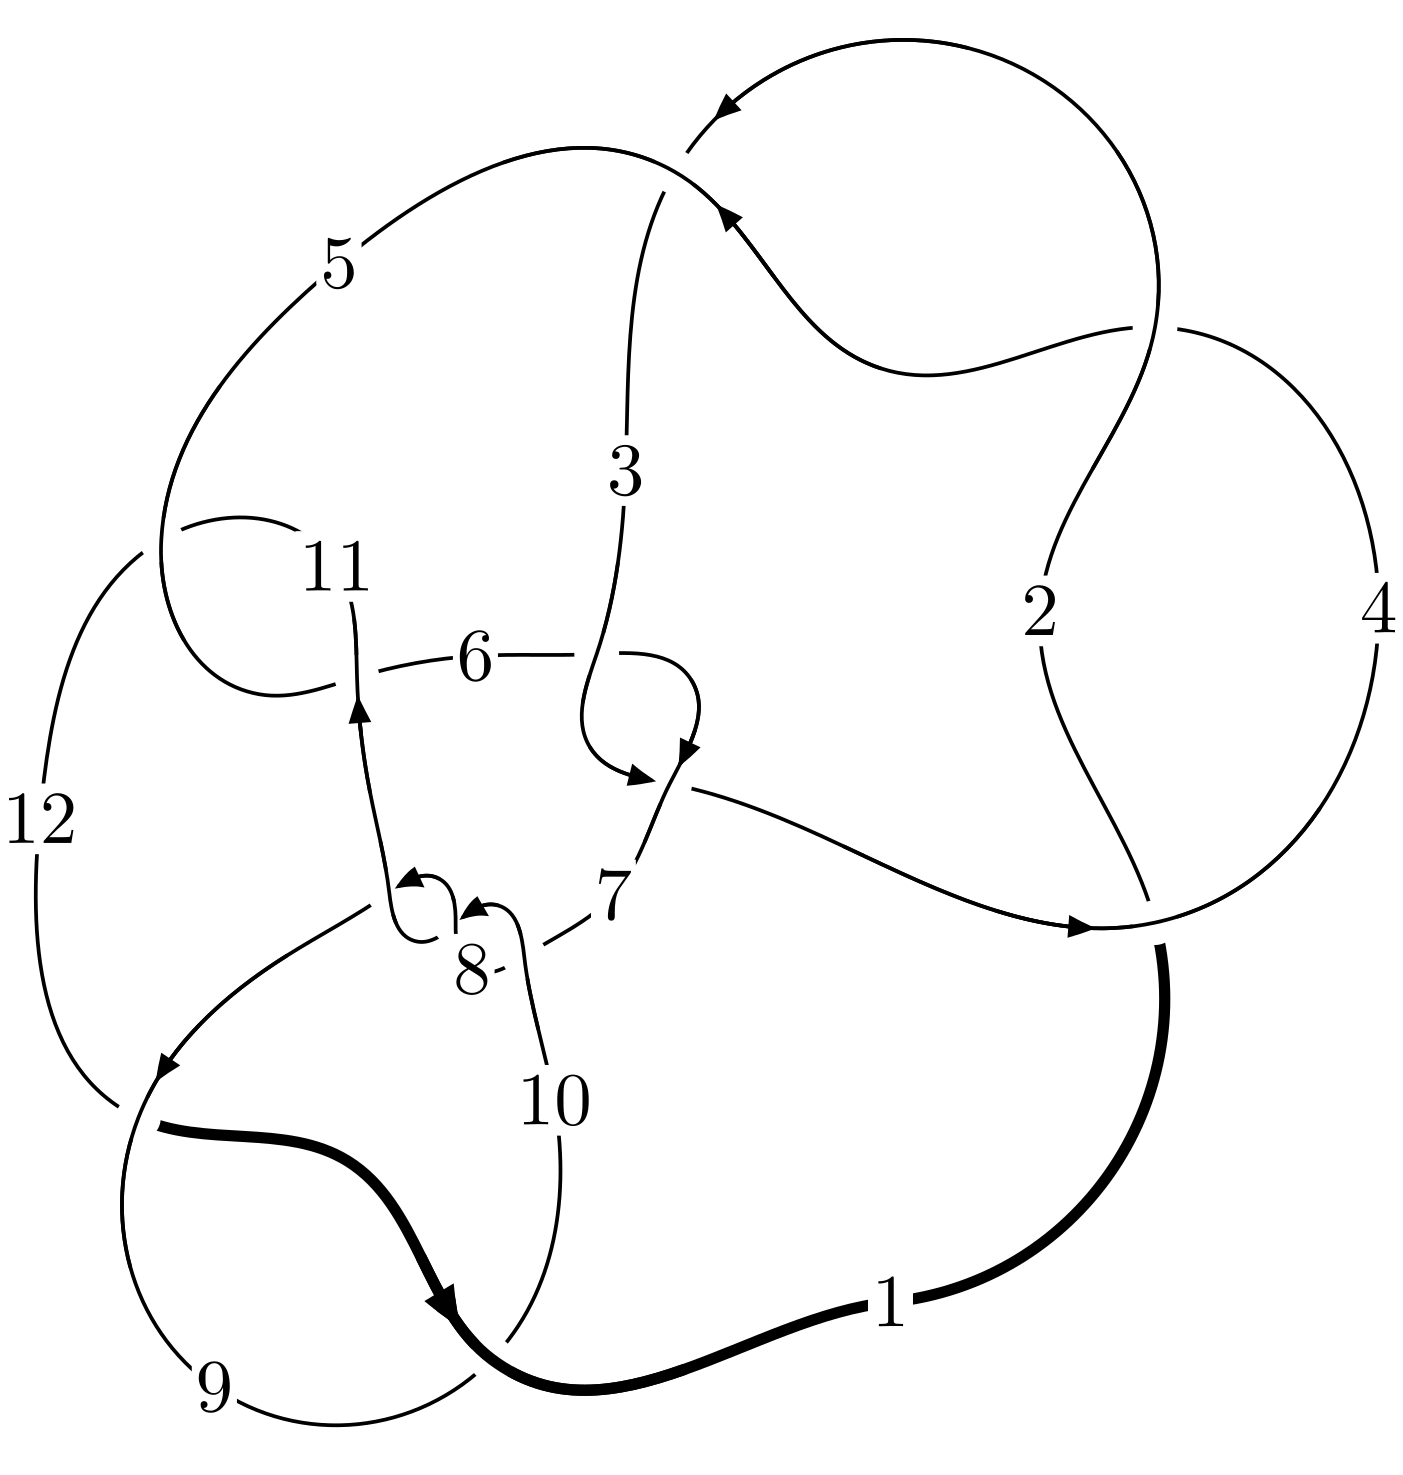
\includegraphics[width=112pt]{../../../GIT/diagram.site/Diagrams/png/2771_12n_0682.png}\\
\ \ \ A knot diagram\footnotemark}&
\allowdisplaybreaks
\textbf{Linearized knot diagam} \\
\cline{2-2}
 &
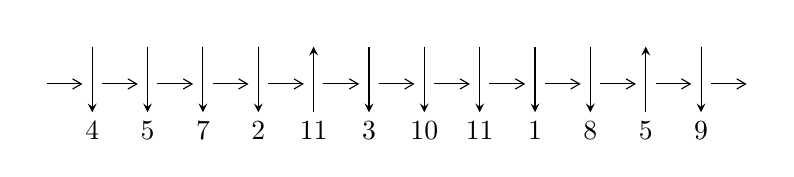
\begin{tikzpicture}[x=20pt, y=17pt]
	% nodes
	\node (C0) at (0, 0) {};
	\node (C1) at (1, 0) {};
	\node (C1U) at (1, +1) {};
	\node (C1D) at (1, -1) {4};

	\node (C2) at (2, 0) {};
	\node (C2U) at (2, +1) {};
	\node (C2D) at (2, -1) {5};

	\node (C3) at (3, 0) {};
	\node (C3U) at (3, +1) {};
	\node (C3D) at (3, -1) {7};

	\node (C4) at (4, 0) {};
	\node (C4U) at (4, +1) {};
	\node (C4D) at (4, -1) {2};

	\node (C5) at (5, 0) {};
	\node (C5U) at (5, +1) {};
	\node (C5D) at (5, -1) {11};

	\node (C6) at (6, 0) {};
	\node (C6U) at (6, +1) {};
	\node (C6D) at (6, -1) {3};

	\node (C7) at (7, 0) {};
	\node (C7U) at (7, +1) {};
	\node (C7D) at (7, -1) {10};

	\node (C8) at (8, 0) {};
	\node (C8U) at (8, +1) {};
	\node (C8D) at (8, -1) {11};

	\node (C9) at (9, 0) {};
	\node (C9U) at (9, +1) {};
	\node (C9D) at (9, -1) {1};

	\node (C10) at (10, 0) {};
	\node (C10U) at (10, +1) {};
	\node (C10D) at (10, -1) {8};

	\node (C11) at (11, 0) {};
	\node (C11U) at (11, +1) {};
	\node (C11D) at (11, -1) {5};

	\node (C12) at (12, 0) {};
	\node (C12U) at (12, +1) {};
	\node (C12D) at (12, -1) {9};
	\node (C13) at (13, 0) {};

	% arrows
	\draw[->,>={angle 60}]
	(C0) edge (C1) (C1) edge (C2) (C2) edge (C3) (C3) edge (C4) (C4) edge (C5) (C5) edge (C6) (C6) edge (C7) (C7) edge (C8) (C8) edge (C9) (C9) edge (C10) (C10) edge (C11) (C11) edge (C12) (C12) edge (C13) ;	\draw[->,>=stealth]
	(C1U) edge (C1D) (C2U) edge (C2D) (C3U) edge (C3D) (C4U) edge (C4D) (C5D) edge (C5U) (C6U) edge (C6D) (C7U) edge (C7D) (C8U) edge (C8D) (C9U) edge (C9D) (C10U) edge (C10D) (C11D) edge (C11U) (C12U) edge (C12D) ;
	\end{tikzpicture} \\
\hhline{~~} \\& 
\textbf{Solving Sequence} \\ \cline{2-2} 
 &
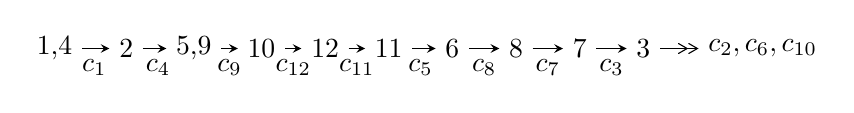
\begin{tikzpicture}[x=23pt, y=7pt]
	% node
	\node (A0) at (-1/8, 0) {1,4};
	\node (A1) at (1, 0) {2};
	\node (A2) at (33/16, 0) {5,9};
	\node (A3) at (25/8, 0) {10};
	\node (A4) at (33/8, 0) {12};
	\node (A5) at (41/8, 0) {11};
	\node (A6) at (49/8, 0) {6};
	\node (A7) at (57/8, 0) {8};
	\node (A8) at (65/8, 0) {7};
	\node (A9) at (73/8, 0) {3};
	\node (C1) at (1/2, -1) {$c_{1}$};
	\node (C2) at (3/2, -1) {$c_{4}$};
	\node (C3) at (21/8, -1) {$c_{9}$};
	\node (C4) at (29/8, -1) {$c_{12}$};
	\node (C5) at (37/8, -1) {$c_{11}$};
	\node (C6) at (45/8, -1) {$c_{5}$};
	\node (C7) at (53/8, -1) {$c_{8}$};
	\node (C8) at (61/8, -1) {$c_{7}$};
	\node (C9) at (69/8, -1) {$c_{3}$};
	\node (A10) at (11, 0) {$c_{2},c_{6},c_{10}$};

	% edge
	\draw[->,>=stealth]	
	(A0) edge (A1) (A1) edge (A2) (A2) edge (A3) (A3) edge (A4) (A4) edge (A5) (A5) edge (A6) (A6) edge (A7) (A7) edge (A8) (A8) edge (A9) ;
	\draw[->>,>={angle 60}]	
	(A9) edge (A10);
\end{tikzpicture} \\ 

\end{tabular} \\

\footnotetext{
The image of knot diagram is generated by the software ``\textbf{Draw programme}" developed by Andrew Bartholomew(\url{http://www.layer8.co.uk/maths/draw/index.htm\#Running-draw}), where we modified some parts for our purpose(\url{https://github.com/CATsTAILs/LinksPainter}).
}\phantom \\ \newline 
\centering \textbf{Ideals for irreducible components\footnotemark of $X_{\text{par}}$} 
 
\begin{align*}
I^u_{1}&=\langle 
u^{12}+2 u^{11}-4 u^{10}-8 u^9+6 u^8+9 u^7-6 u^6+u^5+5 u^4-6 u^3-2 u^2+2 b+3 u,\\
\phantom{I^u_{1}}&\phantom{= \langle  }3 u^{12}+9 u^{11}-22 u^9-16 u^8+5 u^7+5 u^6+11 u^5+20 u^4+9 u^3-2 u^2+2 a-3 u-1,\\
\phantom{I^u_{1}}&\phantom{= \langle  }u^{13}+3 u^{12}- u^{11}-10 u^{10}-4 u^9+9 u^8+3 u^7+8 u^5-7 u^3- u^2+u-1\rangle \\
I^u_{2}&=\langle 
2.01428\times10^{42} u^{43}+5.41774\times10^{42} u^{42}+\cdots+7.34448\times10^{41} b-8.38901\times10^{41},\\
\phantom{I^u_{2}}&\phantom{= \langle  }8.61708\times10^{41} u^{43}+1.60924\times10^{42} u^{42}+\cdots+7.34448\times10^{41} a-4.49822\times10^{43},\;u^{44}+4 u^{43}+\cdots+116 u-1\rangle \\
I^u_{3}&=\langle 
b,\;-3 u^2+a-5 u-4,\;u^3+u^2-1\rangle \\
I^u_{4}&=\langle 
-4 a^2+23 b-33 a-3,\;a^3+8 a^2+3 a+7,\;u-1\rangle \\
I^u_{5}&=\langle 
b+u,\;a+u,\;u^2+u-1\rangle \\
I^u_{6}&=\langle 
b- u-1,\;a+2,\;u^2+u-1\rangle \\
\\
\end{align*}
\raggedright * 6 irreducible components of $\dim_{\mathbb{C}}=0$, with total 67 representations.\\
\footnotetext{All coefficients of polynomials are rational numbers. But the coefficients are sometimes approximated in decimal forms when there is not enough margin.}
\newpage
\renewcommand{\arraystretch}{1}
\centering \section*{I. $I^u_{1}= \langle u^{12}+2 u^{11}+\cdots+2 b+3 u,\;3 u^{12}+9 u^{11}+\cdots+2 a-1,\;u^{13}+3 u^{12}+\cdots+u-1 \rangle$}
\flushleft \textbf{(i) Arc colorings}\\
\begin{tabular}{m{7pt} m{180pt} m{7pt} m{180pt} }
\flushright $a_{1}=$&$\begin{pmatrix}1\\0\end{pmatrix}$ \\
\flushright $a_{4}=$&$\begin{pmatrix}0\\u\end{pmatrix}$ \\
\flushright $a_{2}=$&$\begin{pmatrix}1\\u^2\end{pmatrix}$ \\
\flushright $a_{5}=$&$\begin{pmatrix}- u\\- u^3+u\end{pmatrix}$ \\
\flushright $a_{9}=$&$\begin{pmatrix}-\frac{3}{2} u^{12}-\frac{9}{2} u^{11}+\cdots+\frac{3}{2} u+\frac{1}{2}\\-\frac{1}{2} u^{12}- u^{11}+\cdots+u^2-\frac{3}{2} u\end{pmatrix}$ \\
\flushright $a_{10}=$&$\begin{pmatrix}- u^{12}-\frac{7}{2} u^{11}+\cdots+3 u+\frac{1}{2}\\-\frac{1}{2} u^{12}- u^{11}+\cdots+u^2-\frac{3}{2} u\end{pmatrix}$ \\
\flushright $a_{12}=$&$\begin{pmatrix}-\frac{1}{2} u^{12}-2 u^{11}+\cdots+\frac{3}{2} u+1\\u^3- u\end{pmatrix}$ \\
\flushright $a_{11}=$&$\begin{pmatrix}- u^{11}-2 u^{10}+2 u^9+6 u^8+u^7-3 u^6-2 u^5-3 u^4-3 u^3+2 u+1\\\frac{1}{2} u^{12}+\frac{1}{2} u^{11}+\cdots-\frac{1}{2} u-\frac{1}{2}\end{pmatrix}$ \\
\flushright $a_{6}=$&$\begin{pmatrix}\frac{1}{2} u^{12}-3 u^{10}+\cdots+\frac{3}{2} u-1\\\frac{3}{2} u^{12}+\frac{7}{2} u^{11}+\cdots+\frac{7}{2} u-\frac{3}{2}\end{pmatrix}$ \\
\flushright $a_{8}=$&$\begin{pmatrix}-\frac{1}{2} u^{12}-\frac{5}{2} u^{11}+\cdots+\frac{1}{2} u+\frac{1}{2}\\\frac{1}{2} u^{12}+\frac{1}{2} u^{11}+\cdots-\frac{1}{2} u-\frac{1}{2}\end{pmatrix}$ \\
\flushright $a_{7}=$&$\begin{pmatrix}\frac{1}{2} u^{11}+u^{10}+\cdots- u+\frac{3}{2}\\- u^{11}- u^{10}+4 u^9+3 u^8-6 u^7- u^6+3 u^5-4 u^4+u^3+3 u^2- u\end{pmatrix}$ \\
\flushright $a_{3}=$&$\begin{pmatrix}- u^2+1\\- u^4+2 u^2\end{pmatrix}$\\&\end{tabular}
\flushleft \textbf{(ii) Obstruction class $= -1$}\\~\\
\flushleft \textbf{(iii) Cusp Shapes $= -3 u^{12}-18 u^{11}-24 u^{10}+32 u^9+80 u^8+9 u^7-34 u^6+5 u^5-47 u^4-70 u^3+6 u^2+11 u-18$}\\~\\
\newpage\renewcommand{\arraystretch}{1}
\flushleft \textbf{(iv) u-Polynomials at the component}\newline \\
\begin{tabular}{m{50pt}|m{274pt}}
Crossings & \hspace{64pt}u-Polynomials at each crossing \\
\hline $$\begin{aligned}c_{1},c_{2},c_{4}\\c_{7},c_{8},c_{10}\end{aligned}$$&$\begin{aligned}
&u^{13}-3 u^{12}- u^{11}+10 u^{10}-4 u^9-9 u^8+3 u^7+8 u^5-7 u^3+u^2+u+1
\end{aligned}$\\
\hline $$\begin{aligned}c_{3},c_{6},c_{9}\\c_{12}\end{aligned}$$&$\begin{aligned}
&u^{13}+u^{12}+\cdots+5 u+1
\end{aligned}$\\
\hline $$\begin{aligned}c_{5},c_{11}\end{aligned}$$&$\begin{aligned}
&u^{13}+5 u^{12}+\cdots-8 u-4
\end{aligned}$\\
\hline
\end{tabular}\\~\\
\newpage\renewcommand{\arraystretch}{1}
\flushleft \textbf{(v) Riley Polynomials at the component}\newline \\
\begin{tabular}{m{50pt}|m{274pt}}
Crossings & \hspace{64pt}Riley Polynomials at each crossing \\
\hline $$\begin{aligned}c_{1},c_{2},c_{4}\\c_{7},c_{8},c_{10}\end{aligned}$$&$\begin{aligned}
&y^{13}-11 y^{12}+\cdots- y-1
\end{aligned}$\\
\hline $$\begin{aligned}c_{3},c_{6},c_{9}\\c_{12}\end{aligned}$$&$\begin{aligned}
&y^{13}-3 y^{12}+\cdots+7 y-1
\end{aligned}$\\
\hline $$\begin{aligned}c_{5},c_{11}\end{aligned}$$&$\begin{aligned}
&y^{13}-5 y^{12}+\cdots+96 y-16
\end{aligned}$\\
\hline
\end{tabular}\\~\\
\newpage\flushleft \textbf{(vi) Complex Volumes and Cusp Shapes}
$$\begin{array}{c|c|c}  
\text{Solutions to }I^u_{1}& \I (\text{vol} + \sqrt{-1}CS) & \text{Cusp shape}\\
 \hline 
\begin{aligned}
u &= \phantom{-}0.920255\phantom{ +0.000000I} \\
a &= -7.53293\phantom{ +0.000000I} \\
b &= -0.375392\phantom{ +0.000000I}\end{aligned}
 & -2.84609\phantom{ +0.000000I} & -65.8580\phantom{ +0.000000I} \\ \hline\begin{aligned}
u &= \phantom{-}0.217488 + 0.883339 I \\
a &= \phantom{-}0.447419 - 0.357015 I \\
b &= \phantom{-}1.079610 + 0.670263 I\end{aligned}
 & \phantom{-}2.14237 - 5.68500 I & -7.77978 + 6.07128 I \\ \hline\begin{aligned}
u &= \phantom{-}0.217488 - 0.883339 I \\
a &= \phantom{-}0.447419 + 0.357015 I \\
b &= \phantom{-}1.079610 - 0.670263 I\end{aligned}
 & \phantom{-}2.14237 + 5.68500 I & -7.77978 - 6.07128 I \\ \hline\begin{aligned}
u &= -0.795282 + 0.405757 I \\
a &= -0.416083 + 0.498754 I \\
b &= -0.175698 + 0.846144 I\end{aligned}
 & \phantom{-}1.52283 + 3.56370 I & -3.66796 - 8.41026 I \\ \hline\begin{aligned}
u &= -0.795282 - 0.405757 I \\
a &= -0.416083 - 0.498754 I \\
b &= -0.175698 - 0.846144 I\end{aligned}
 & \phantom{-}1.52283 - 3.56370 I & -3.66796 + 8.41026 I \\ \hline\begin{aligned}
u &= \phantom{-}1.266340 + 0.164860 I \\
a &= -1.095680 + 0.368409 I \\
b &= -0.352007 + 0.886032 I\end{aligned}
 & -3.86762 - 1.80054 I & -11.65148 + 0.61379 I \\ \hline\begin{aligned}
u &= \phantom{-}1.266340 - 0.164860 I \\
a &= -1.095680 - 0.368409 I \\
b &= -0.352007 - 0.886032 I\end{aligned}
 & -3.86762 + 1.80054 I & -11.65148 - 0.61379 I \\ \hline\begin{aligned}
u &= -1.38670 + 0.37744 I \\
a &= \phantom{-}1.155750 + 0.361386 I \\
b &= \phantom{-}1.132190 - 0.771142 I\end{aligned}
 & -10.71940 + 7.71547 I & -15.7360 - 5.7316 I \\ \hline\begin{aligned}
u &= -1.38670 - 0.37744 I \\
a &= \phantom{-}1.155750 - 0.361386 I \\
b &= \phantom{-}1.132190 + 0.771142 I\end{aligned}
 & -10.71940 - 7.71547 I & -15.7360 + 5.7316 I \\ \hline\begin{aligned}
u &= \phantom{-}0.240304 + 0.377267 I \\
a &= \phantom{-}1.36715 + 1.11084 I \\
b &= -0.640664 - 0.285334 I\end{aligned}
 & -0.98403 - 1.11558 I & -8.69395 + 6.01211 I\\
 \hline 
 \end{array}$$\newpage$$\begin{array}{c|c|c}  
\text{Solutions to }I^u_{1}& \I (\text{vol} + \sqrt{-1}CS) & \text{Cusp shape}\\
 \hline 
\begin{aligned}
u &= \phantom{-}0.240304 - 0.377267 I \\
a &= \phantom{-}1.36715 - 1.11084 I \\
b &= -0.640664 + 0.285334 I\end{aligned}
 & -0.98403 + 1.11558 I & -8.69395 - 6.01211 I \\ \hline\begin{aligned}
u &= -1.50228 + 0.43298 I \\
a &= -1.69209 - 0.37137 I \\
b &= -1.35574 + 0.89152 I\end{aligned}
 & -8.8777 + 15.5620 I & -14.5417 - 7.8795 I \\ \hline\begin{aligned}
u &= -1.50228 - 0.43298 I \\
a &= -1.69209 + 0.37137 I \\
b &= -1.35574 - 0.89152 I\end{aligned}
 & -8.8777 - 15.5620 I & -14.5417 + 7.8795 I\\
 \hline 
 \end{array}$$\newpage\newpage\renewcommand{\arraystretch}{1}
\centering \section*{II. $I^u_{2}= \langle 2.01\times10^{42} u^{43}+5.42\times10^{42} u^{42}+\cdots+7.34\times10^{41} b-8.39\times10^{41},\;8.62\times10^{41} u^{43}+1.61\times10^{42} u^{42}+\cdots+7.34\times10^{41} a-4.50\times10^{43},\;u^{44}+4 u^{43}+\cdots+116 u-1 \rangle$}
\flushleft \textbf{(i) Arc colorings}\\
\begin{tabular}{m{7pt} m{180pt} m{7pt} m{180pt} }
\flushright $a_{1}=$&$\begin{pmatrix}1\\0\end{pmatrix}$ \\
\flushright $a_{4}=$&$\begin{pmatrix}0\\u\end{pmatrix}$ \\
\flushright $a_{2}=$&$\begin{pmatrix}1\\u^2\end{pmatrix}$ \\
\flushright $a_{5}=$&$\begin{pmatrix}- u\\- u^3+u\end{pmatrix}$ \\
\flushright $a_{9}=$&$\begin{pmatrix}-1.17327 u^{43}-2.19108 u^{42}+\cdots-439.275 u+61.2463\\-2.74257 u^{43}-7.37661 u^{42}+\cdots-201.685 u+1.14222\end{pmatrix}$ \\
\flushright $a_{10}=$&$\begin{pmatrix}1.56930 u^{43}+5.18553 u^{42}+\cdots-237.590 u+60.1040\\-2.74257 u^{43}-7.37661 u^{42}+\cdots-201.685 u+1.14222\end{pmatrix}$ \\
\flushright $a_{12}=$&$\begin{pmatrix}3.61816 u^{43}+9.27065 u^{42}+\cdots+182.489 u+32.8026\\4.49904 u^{43}+11.8002 u^{42}+\cdots+312.338 u-3.00702\end{pmatrix}$ \\
\flushright $a_{11}=$&$\begin{pmatrix}1.96942 u^{43}+5.25944 u^{42}+\cdots+65.5876 u+33.8026\\2.07745 u^{43}+5.75738 u^{42}+\cdots+127.873 u-1.42316\end{pmatrix}$ \\
\flushright $a_{6}=$&$\begin{pmatrix}1.07148 u^{43}+2.89399 u^{42}+\cdots+59.4605 u+9.96375\\1.37364 u^{43}+3.38028 u^{42}+\cdots+86.1371 u-0.830453\end{pmatrix}$ \\
\flushright $a_{8}=$&$\begin{pmatrix}1.70871 u^{43}+4.01744 u^{42}+\cdots+60.7021 u+31.6372\\2.07745 u^{43}+5.75738 u^{42}+\cdots+127.873 u-1.42316\end{pmatrix}$ \\
\flushright $a_{7}=$&$\begin{pmatrix}1.78926 u^{43}+4.62600 u^{42}+\cdots+163.701 u-11.9689\\-1.22781 u^{43}-2.74973 u^{42}+\cdots-70.8975 u+0.701920\end{pmatrix}$ \\
\flushright $a_{3}=$&$\begin{pmatrix}- u^2+1\\- u^4+2 u^2\end{pmatrix}$\\&\end{tabular}
\flushleft \textbf{(ii) Obstruction class $= -1$}\\~\\
\flushleft \textbf{(iii) Cusp Shapes $= -2.60530 u^{43}-11.0854 u^{42}+\cdots+553.011 u-13.5461$}\\~\\
\newpage\renewcommand{\arraystretch}{1}
\flushleft \textbf{(iv) u-Polynomials at the component}\newline \\
\begin{tabular}{m{50pt}|m{274pt}}
Crossings & \hspace{64pt}u-Polynomials at each crossing \\
\hline $$\begin{aligned}c_{1},c_{2},c_{4}\\c_{7},c_{8},c_{10}\end{aligned}$$&$\begin{aligned}
&u^{44}-4 u^{43}+\cdots-116 u-1
\end{aligned}$\\
\hline $$\begin{aligned}c_{3},c_{6},c_{9}\\c_{12}\end{aligned}$$&$\begin{aligned}
&u^{44}+3 u^{43}+\cdots-44 u+8
\end{aligned}$\\
\hline $$\begin{aligned}c_{5},c_{11}\end{aligned}$$&$\begin{aligned}
&(u^{22}- u^{21}+\cdots-9 u-2)^{2}
\end{aligned}$\\
\hline
\end{tabular}\\~\\
\newpage\renewcommand{\arraystretch}{1}
\flushleft \textbf{(v) Riley Polynomials at the component}\newline \\
\begin{tabular}{m{50pt}|m{274pt}}
Crossings & \hspace{64pt}Riley Polynomials at each crossing \\
\hline $$\begin{aligned}c_{1},c_{2},c_{4}\\c_{7},c_{8},c_{10}\end{aligned}$$&$\begin{aligned}
&y^{44}-40 y^{43}+\cdots-12428 y+1
\end{aligned}$\\
\hline $$\begin{aligned}c_{3},c_{6},c_{9}\\c_{12}\end{aligned}$$&$\begin{aligned}
&y^{44}-21 y^{43}+\cdots-7760 y+64
\end{aligned}$\\
\hline $$\begin{aligned}c_{5},c_{11}\end{aligned}$$&$\begin{aligned}
&(y^{22}-15 y^{21}+\cdots-113 y+4)^{2}
\end{aligned}$\\
\hline
\end{tabular}\\~\\
\newpage\flushleft \textbf{(vi) Complex Volumes and Cusp Shapes}
$$\begin{array}{c|c|c}  
\text{Solutions to }I^u_{2}& \I (\text{vol} + \sqrt{-1}CS) & \text{Cusp shape}\\
 \hline 
\begin{aligned}
u &= \phantom{-}1.090540 + 0.022158 I \\
a &= -3.21063 - 2.07089 I \\
b &= -0.729158 - 0.031613 I\end{aligned}
 & -2.83824 + 0.14755 I & -2.77483 - 4.21375 I \\ \hline\begin{aligned}
u &= \phantom{-}1.090540 - 0.022158 I \\
a &= -3.21063 + 2.07089 I \\
b &= -0.729158 + 0.031613 I\end{aligned}
 & -2.83824 - 0.14755 I & -2.77483 + 4.21375 I \\ \hline\begin{aligned}
u &= \phantom{-}0.109119 + 0.888646 I \\
a &= -0.410159 - 0.255099 I \\
b &= \phantom{-}1.061150 + 0.336334 I\end{aligned}
 & -5.93215 - 3.14286 I & -14.6418 + 3.7109 I \\ \hline\begin{aligned}
u &= \phantom{-}0.109119 - 0.888646 I \\
a &= -0.410159 + 0.255099 I \\
b &= \phantom{-}1.061150 - 0.336334 I\end{aligned}
 & -5.93215 + 3.14286 I & -14.6418 - 3.7109 I \\ \hline\begin{aligned}
u &= \phantom{-}0.344224 + 1.065750 I \\
a &= -0.392445 + 0.502444 I \\
b &= -1.174950 - 0.756583 I\end{aligned}
 & -3.01557 - 10.18830 I & -12.15400 + 6.99410 I \\ \hline\begin{aligned}
u &= \phantom{-}0.344224 - 1.065750 I \\
a &= -0.392445 - 0.502444 I \\
b &= -1.174950 + 0.756583 I\end{aligned}
 & -3.01557 + 10.18830 I & -12.15400 - 6.99410 I \\ \hline\begin{aligned}
u &= -1.134110 + 0.122816 I \\
a &= -0.077142 + 0.931712 I \\
b &= \phantom{-}0.03859 + 1.46465 I\end{aligned}
 & \phantom{-}1.18895 + 3.23778 I & -15.5021 - 9.5411 I \\ \hline\begin{aligned}
u &= -1.134110 - 0.122816 I \\
a &= -0.077142 - 0.931712 I \\
b &= \phantom{-}0.03859 - 1.46465 I\end{aligned}
 & \phantom{-}1.18895 - 3.23778 I & -15.5021 + 9.5411 I \\ \hline\begin{aligned}
u &= \phantom{-}1.036890 + 0.519128 I \\
a &= \phantom{-}0.495432 - 0.747200 I \\
b &= \phantom{-}0.705965 - 0.517769 I\end{aligned}
 & -0.357526 + 0.716312 I & -8.85937 - 2.91987 I \\ \hline\begin{aligned}
u &= \phantom{-}1.036890 - 0.519128 I \\
a &= \phantom{-}0.495432 + 0.747200 I \\
b &= \phantom{-}0.705965 + 0.517769 I\end{aligned}
 & -0.357526 - 0.716312 I & -8.85937 + 2.91987 I\\
 \hline 
 \end{array}$$\newpage$$\begin{array}{c|c|c}  
\text{Solutions to }I^u_{2}& \I (\text{vol} + \sqrt{-1}CS) & \text{Cusp shape}\\
 \hline 
\begin{aligned}
u &= -0.748799 + 0.898808 I \\
a &= -0.318628 - 0.160414 I \\
b &= -0.598618 + 0.291695 I\end{aligned}
 & \phantom{-}1.18895 + 3.23778 I & -15.5021 - 9.5411 I \\ \hline\begin{aligned}
u &= -0.748799 - 0.898808 I \\
a &= -0.318628 + 0.160414 I \\
b &= -0.598618 - 0.291695 I\end{aligned}
 & \phantom{-}1.18895 - 3.23778 I & -15.5021 + 9.5411 I \\ \hline\begin{aligned}
u &= \phantom{-}0.238284 + 0.726491 I \\
a &= -0.590561 - 1.081680 I \\
b &= -0.583355 + 1.078870 I\end{aligned}
 & -1.09298 - 3.55787 I & -9.79859 + 4.38747 I \\ \hline\begin{aligned}
u &= \phantom{-}0.238284 - 0.726491 I \\
a &= -0.590561 + 1.081680 I \\
b &= -0.583355 - 1.078870 I\end{aligned}
 & -1.09298 + 3.55787 I & -9.79859 - 4.38747 I \\ \hline\begin{aligned}
u &= \phantom{-}0.736176\phantom{ +0.000000I} \\
a &= \phantom{-}0.801410\phantom{ +0.000000I} \\
b &= \phantom{-}0.0947175\phantom{ +0.000000I}\end{aligned}
 & -1.10346\phantom{ +0.000000I} & -8.70720\phantom{ +0.000000I} \\ \hline\begin{aligned}
u &= -0.164222 + 0.700108 I \\
a &= \phantom{-}0.889479 + 0.479637 I \\
b &= \phantom{-}0.576121 - 0.856265 I\end{aligned}
 & \phantom{-}3.71629\phantom{ +0.000000I} & -3.80483 + 0. I\phantom{ +0.000000I} \\ \hline\begin{aligned}
u &= -0.164222 - 0.700108 I \\
a &= \phantom{-}0.889479 - 0.479637 I \\
b &= \phantom{-}0.576121 + 0.856265 I\end{aligned}
 & \phantom{-}3.71629\phantom{ +0.000000I} & -3.80483 + 0. I\phantom{ +0.000000I} \\ \hline\begin{aligned}
u &= \phantom{-}1.243520 + 0.352072 I \\
a &= \phantom{-}0.852793 - 1.120250 I \\
b &= \phantom{-}1.274130 + 0.140265 I\end{aligned}
 & -9.47192 - 1.36166 I & \phantom{-0.000000 } 0 \\ \hline\begin{aligned}
u &= \phantom{-}1.243520 - 0.352072 I \\
a &= \phantom{-}0.852793 + 1.120250 I \\
b &= \phantom{-}1.274130 - 0.140265 I\end{aligned}
 & -9.47192 + 1.36166 I & \phantom{-0.000000 } 0 \\ \hline\begin{aligned}
u &= \phantom{-}0.643688 + 0.282110 I \\
a &= -2.22845 + 4.03294 I \\
b &= -0.062262 - 0.456825 I\end{aligned}
 & -2.83824 - 0.14755 I & -2.77483 + 4.21375 I\\
 \hline 
 \end{array}$$\newpage$$\begin{array}{c|c|c}  
\text{Solutions to }I^u_{2}& \I (\text{vol} + \sqrt{-1}CS) & \text{Cusp shape}\\
 \hline 
\begin{aligned}
u &= \phantom{-}0.643688 - 0.282110 I \\
a &= -2.22845 - 4.03294 I \\
b &= -0.062262 + 0.456825 I\end{aligned}
 & -2.83824 + 0.14755 I & -2.77483 - 4.21375 I \\ \hline\begin{aligned}
u &= \phantom{-}1.047760 + 0.864022 I \\
a &= -0.255518 + 0.521043 I \\
b &= -1.055110 + 0.486781 I\end{aligned}
 & -5.02280 + 3.68716 I & \phantom{-0.000000 } 0 \\ \hline\begin{aligned}
u &= \phantom{-}1.047760 - 0.864022 I \\
a &= -0.255518 - 0.521043 I \\
b &= -1.055110 - 0.486781 I\end{aligned}
 & -5.02280 - 3.68716 I & \phantom{-0.000000 } 0 \\ \hline\begin{aligned}
u &= -1.351490 + 0.160264 I \\
a &= -1.139470 - 0.246938 I \\
b &= -0.991832 + 0.785748 I\end{aligned}
 & -5.93215 + 3.14286 I & \phantom{-0.000000 } 0 \\ \hline\begin{aligned}
u &= -1.351490 - 0.160264 I \\
a &= -1.139470 + 0.246938 I \\
b &= -0.991832 - 0.785748 I\end{aligned}
 & -5.93215 - 3.14286 I & \phantom{-0.000000 } 0 \\ \hline\begin{aligned}
u &= -1.347140 + 0.234013 I \\
a &= -2.04959 - 0.19598 I \\
b &= -1.55821 + 0.42887 I\end{aligned}
 & -5.02280 + 3.68716 I & \phantom{-0.000000 } 0 \\ \hline\begin{aligned}
u &= -1.347140 - 0.234013 I \\
a &= -2.04959 + 0.19598 I \\
b &= -1.55821 - 0.42887 I\end{aligned}
 & -5.02280 - 3.68716 I & \phantom{-0.000000 } 0 \\ \hline\begin{aligned}
u &= \phantom{-}1.358520 + 0.282419 I \\
a &= \phantom{-}1.96744 - 0.07093 I \\
b &= \phantom{-}0.937408 + 0.526012 I\end{aligned}
 & -1.09298 - 3.55787 I & \phantom{-0.000000 } 0 \\ \hline\begin{aligned}
u &= \phantom{-}1.358520 - 0.282419 I \\
a &= \phantom{-}1.96744 + 0.07093 I \\
b &= \phantom{-}0.937408 - 0.526012 I\end{aligned}
 & -1.09298 + 3.55787 I & \phantom{-0.000000 } 0 \\ \hline\begin{aligned}
u &= \phantom{-}0.117503 + 0.569726 I \\
a &= -0.457122 - 0.216490 I \\
b &= -1.007210 - 0.504052 I\end{aligned}
 & -0.357526 - 0.716312 I & -8.85937 + 2.91987 I\\
 \hline 
 \end{array}$$\newpage$$\begin{array}{c|c|c}  
\text{Solutions to }I^u_{2}& \I (\text{vol} + \sqrt{-1}CS) & \text{Cusp shape}\\
 \hline 
\begin{aligned}
u &= \phantom{-}0.117503 - 0.569726 I \\
a &= -0.457122 + 0.216490 I \\
b &= -1.007210 + 0.504052 I\end{aligned}
 & -0.357526 + 0.716312 I & -8.85937 - 2.91987 I \\ \hline\begin{aligned}
u &= -1.42436\phantom{ +0.000000I} \\
a &= \phantom{-}2.09618\phantom{ +0.000000I} \\
b &= \phantom{-}2.01618\phantom{ +0.000000I}\end{aligned}
 & -16.0009\phantom{ +0.000000I} & \phantom{-0.000000 } 0 \\ \hline\begin{aligned}
u &= -1.39535 + 0.29610 I \\
a &= -0.197837 - 0.800968 I \\
b &= -0.58639 - 1.50954 I\end{aligned}
 & -6.28468 + 7.27868 I & \phantom{-0.000000 } 0 \\ \hline\begin{aligned}
u &= -1.39535 - 0.29610 I \\
a &= -0.197837 + 0.800968 I \\
b &= -0.58639 + 1.50954 I\end{aligned}
 & -6.28468 - 7.27868 I & \phantom{-0.000000 } 0 \\ \hline\begin{aligned}
u &= -1.40825 + 0.36939 I \\
a &= \phantom{-}1.88459 + 0.34782 I \\
b &= \phantom{-}1.39293 - 0.68109 I\end{aligned}
 & -3.01557 + 10.18830 I & \phantom{-0.000000 } 0 \\ \hline\begin{aligned}
u &= -1.40825 - 0.36939 I \\
a &= \phantom{-}1.88459 - 0.34782 I \\
b &= \phantom{-}1.39293 + 0.68109 I\end{aligned}
 & -3.01557 - 10.18830 I & \phantom{-0.000000 } 0 \\ \hline\begin{aligned}
u &= -1.45462 + 0.06689 I \\
a &= \phantom{-}0.830038 - 0.316230 I \\
b &= \phantom{-}0.720926 + 0.858306 I\end{aligned}
 & -9.47192 + 1.36166 I & \phantom{-0.000000 } 0 \\ \hline\begin{aligned}
u &= -1.45462 - 0.06689 I \\
a &= \phantom{-}0.830038 + 0.316230 I \\
b &= \phantom{-}0.720926 - 0.858306 I\end{aligned}
 & -9.47192 - 1.36166 I & \phantom{-0.000000 } 0 \\ \hline\begin{aligned}
u &= \phantom{-}0.521744\phantom{ +0.000000I} \\
a &= -2.11947\phantom{ +0.000000I} \\
b &= \phantom{-}1.64818\phantom{ +0.000000I}\end{aligned}
 & -9.78452\phantom{ +0.000000I} & \phantom{-}30.1490\phantom{ +0.000000I} \\ \hline\begin{aligned}
u &= \phantom{-}1.57069 + 0.28000 I \\
a &= -1.52006 + 0.01103 I \\
b &= -1.152160 - 0.610789 I\end{aligned}
 & -6.28468 - 7.27868 I & \phantom{-0.000000 } 0\\
 \hline 
 \end{array}$$\newpage$$\begin{array}{c|c|c}  
\text{Solutions to }I^u_{2}& \I (\text{vol} + \sqrt{-1}CS) & \text{Cusp shape}\\
 \hline 
\begin{aligned}
u &= \phantom{-}1.57069 - 0.28000 I \\
a &= -1.52006 - 0.01103 I \\
b &= -1.152160 + 0.610789 I\end{aligned}
 & -6.28468 + 7.27868 I & \phantom{-0.000000 } 0 \\ \hline\begin{aligned}
u &= -1.63226\phantom{ +0.000000I} \\
a &= \phantom{-}1.82053\phantom{ +0.000000I} \\
b &= \phantom{-}0.616211\phantom{ +0.000000I}\end{aligned}
 & -9.78452\phantom{ +0.000000I} & \phantom{-0.000000 } 0 \\ \hline\begin{aligned}
u &= -1.80378\phantom{ +0.000000I} \\
a &= -1.14737\phantom{ +0.000000I} \\
b &= -1.21054\phantom{ +0.000000I}\end{aligned}
 & -16.0009\phantom{ +0.000000I} & \phantom{-0.000000 } 0 \\ \hline\begin{aligned}
u &= \phantom{-}0.00897213\phantom{ +0.000000I} \\
a &= \phantom{-}57.4044\phantom{ +0.000000I} \\
b &= -0.580690\phantom{ +0.000000I}\end{aligned}
 & -1.10346\phantom{ +0.000000I} & -8.70720\phantom{ +0.000000I}\\
 \hline 
 \end{array}$$\newpage\newpage\renewcommand{\arraystretch}{1}
\centering \section*{III. $I^u_{3}= \langle b,\;-3 u^2+a-5 u-4,\;u^3+u^2-1 \rangle$}
\flushleft \textbf{(i) Arc colorings}\\
\begin{tabular}{m{7pt} m{180pt} m{7pt} m{180pt} }
\flushright $a_{1}=$&$\begin{pmatrix}1\\0\end{pmatrix}$ \\
\flushright $a_{4}=$&$\begin{pmatrix}0\\u\end{pmatrix}$ \\
\flushright $a_{2}=$&$\begin{pmatrix}1\\u^2\end{pmatrix}$ \\
\flushright $a_{5}=$&$\begin{pmatrix}- u\\u^2+u-1\end{pmatrix}$ \\
\flushright $a_{9}=$&$\begin{pmatrix}3 u^2+5 u+4\\0\end{pmatrix}$ \\
\flushright $a_{10}=$&$\begin{pmatrix}3 u^2+5 u+4\\0\end{pmatrix}$ \\
\flushright $a_{12}=$&$\begin{pmatrix}1\\0\end{pmatrix}$ \\
\flushright $a_{11}=$&$\begin{pmatrix}u\\-2 u^2- u+2\end{pmatrix}$ \\
\flushright $a_{6}=$&$\begin{pmatrix}-2 u+1\\5 u^2+2 u-4\end{pmatrix}$ \\
\flushright $a_{8}=$&$\begin{pmatrix}3 u^2+4 u+4\\2 u^2+u-2\end{pmatrix}$ \\
\flushright $a_{7}=$&$\begin{pmatrix}- u\\2 u^2+u-2\end{pmatrix}$ \\
\flushright $a_{3}=$&$\begin{pmatrix}- u^2+1\\u^2- u+1\end{pmatrix}$\\&\end{tabular}
\flushleft \textbf{(ii) Obstruction class $= 1$}\\~\\
\flushleft \textbf{(iii) Cusp Shapes $= 21 u^2+45 u+27$}\\~\\
\newpage\renewcommand{\arraystretch}{1}
\flushleft \textbf{(iv) u-Polynomials at the component}\newline \\
\begin{tabular}{m{50pt}|m{274pt}}
Crossings & \hspace{64pt}u-Polynomials at each crossing \\
\hline $$\begin{aligned}c_{1},c_{2}\end{aligned}$$&$\begin{aligned}
&u^3+u^2-1
\end{aligned}$\\
\hline $$\begin{aligned}c_{3}\end{aligned}$$&$\begin{aligned}
&u^3- u^2+2 u-1
\end{aligned}$\\
\hline $$\begin{aligned}c_{4}\end{aligned}$$&$\begin{aligned}
&u^3- u^2+1
\end{aligned}$\\
\hline $$\begin{aligned}c_{5}\end{aligned}$$&$\begin{aligned}
&u^3-3 u^2+2 u+1
\end{aligned}$\\
\hline $$\begin{aligned}c_{6}\end{aligned}$$&$\begin{aligned}
&u^3+u^2+2 u+1
\end{aligned}$\\
\hline $$\begin{aligned}c_{7},c_{8}\end{aligned}$$&$\begin{aligned}
&(u-1)^3
\end{aligned}$\\
\hline $$\begin{aligned}c_{9},c_{12}\end{aligned}$$&$\begin{aligned}
&u^3
\end{aligned}$\\
\hline $$\begin{aligned}c_{10}\end{aligned}$$&$\begin{aligned}
&(u+1)^3
\end{aligned}$\\
\hline $$\begin{aligned}c_{11}\end{aligned}$$&$\begin{aligned}
&u^3+3 u^2+2 u-1
\end{aligned}$\\
\hline
\end{tabular}\\~\\
\newpage\renewcommand{\arraystretch}{1}
\flushleft \textbf{(v) Riley Polynomials at the component}\newline \\
\begin{tabular}{m{50pt}|m{274pt}}
Crossings & \hspace{64pt}Riley Polynomials at each crossing \\
\hline $$\begin{aligned}c_{1},c_{2},c_{4}\end{aligned}$$&$\begin{aligned}
&y^3- y^2+2 y-1
\end{aligned}$\\
\hline $$\begin{aligned}c_{3},c_{6}\end{aligned}$$&$\begin{aligned}
&y^3+3 y^2+2 y-1
\end{aligned}$\\
\hline $$\begin{aligned}c_{5},c_{11}\end{aligned}$$&$\begin{aligned}
&y^3-5 y^2+10 y-1
\end{aligned}$\\
\hline $$\begin{aligned}c_{7},c_{8},c_{10}\end{aligned}$$&$\begin{aligned}
&(y-1)^3
\end{aligned}$\\
\hline $$\begin{aligned}c_{9},c_{12}\end{aligned}$$&$\begin{aligned}
&y^3
\end{aligned}$\\
\hline
\end{tabular}\\~\\
\newpage\flushleft \textbf{(vi) Complex Volumes and Cusp Shapes}
$$\begin{array}{c|c|c}  
\text{Solutions to }I^u_{3}& \I (\text{vol} + \sqrt{-1}CS) & \text{Cusp shape}\\
 \hline 
\begin{aligned}
u &= -0.877439 + 0.744862 I \\
a &= \phantom{-}0.258045 - 0.197115 I \\
b &= \phantom{-0.000000 } 0\end{aligned}
 & \phantom{-}1.37919 + 2.82812 I & -7.96807 + 6.06881 I \\ \hline\begin{aligned}
u &= -0.877439 - 0.744862 I \\
a &= \phantom{-}0.258045 + 0.197115 I \\
b &= \phantom{-0.000000 } 0\end{aligned}
 & \phantom{-}1.37919 - 2.82812 I & -7.96807 - 6.06881 I \\ \hline\begin{aligned}
u &= \phantom{-}0.754878\phantom{ +0.000000I} \\
a &= \phantom{-}9.48391\phantom{ +0.000000I} \\
b &= \phantom{-0.000000 } 0\end{aligned}
 & -2.75839\phantom{ +0.000000I} & \phantom{-}72.9360\phantom{ +0.000000I}\\
 \hline 
 \end{array}$$\newpage\newpage\renewcommand{\arraystretch}{1}
\centering \section*{IV. $I^u_{4}= \langle -4 a^2+23 b-33 a-3,\;a^3+8 a^2+3 a+7,\;u-1 \rangle$}
\flushleft \textbf{(i) Arc colorings}\\
\begin{tabular}{m{7pt} m{180pt} m{7pt} m{180pt} }
\flushright $a_{1}=$&$\begin{pmatrix}1\\0\end{pmatrix}$ \\
\flushright $a_{4}=$&$\begin{pmatrix}0\\1\end{pmatrix}$ \\
\flushright $a_{2}=$&$\begin{pmatrix}1\\1\end{pmatrix}$ \\
\flushright $a_{5}=$&$\begin{pmatrix}-1\\0\end{pmatrix}$ \\
\flushright $a_{9}=$&$\begin{pmatrix}a\\\frac{4}{23} a^2+\frac{33}{23} a+\frac{3}{23}\end{pmatrix}$ \\
\flushright $a_{10}=$&$\begin{pmatrix}-\frac{4}{23} a^2-\frac{10}{23} a-\frac{3}{23}\\\frac{4}{23} a^2+\frac{33}{23} a+\frac{3}{23}\end{pmatrix}$ \\
\flushright $a_{12}=$&$\begin{pmatrix}-\frac{1}{23} a^2+\frac{9}{23} a+\frac{51}{23}\\\frac{1}{23} a^2+\frac{14}{23} a+\frac{41}{23}\end{pmatrix}$ \\
\flushright $a_{11}=$&$\begin{pmatrix}-\frac{2}{23} a^2-\frac{5}{23} a+\frac{10}{23}\\\frac{1}{23} a^2+\frac{14}{23} a+\frac{41}{23}\end{pmatrix}$ \\
\flushright $a_{6}=$&$\begin{pmatrix}0\\\frac{5}{23} a^2+\frac{47}{23} a+\frac{67}{23}\end{pmatrix}$ \\
\flushright $a_{8}=$&$\begin{pmatrix}-\frac{1}{23} a^2+\frac{9}{23} a+\frac{5}{23}\\\frac{1}{23} a^2+\frac{14}{23} a+\frac{41}{23}\end{pmatrix}$ \\
\flushright $a_{7}=$&$\begin{pmatrix}0\\\frac{5}{23} a^2+\frac{47}{23} a+\frac{67}{23}\end{pmatrix}$ \\
\flushright $a_{3}=$&$\begin{pmatrix}0\\1\end{pmatrix}$\\&\end{tabular}
\flushleft \textbf{(ii) Obstruction class $= 1$}\\~\\
\flushleft \textbf{(iii) Cusp Shapes $= \frac{51}{23} a^2+\frac{162}{23} a-\frac{117}{23}$}\\~\\
\newpage\renewcommand{\arraystretch}{1}
\flushleft \textbf{(iv) u-Polynomials at the component}\newline \\
\begin{tabular}{m{50pt}|m{274pt}}
Crossings & \hspace{64pt}u-Polynomials at each crossing \\
\hline $$\begin{aligned}c_{1},c_{2}\end{aligned}$$&$\begin{aligned}
&(u-1)^3
\end{aligned}$\\
\hline $$\begin{aligned}c_{3},c_{6}\end{aligned}$$&$\begin{aligned}
&u^3
\end{aligned}$\\
\hline $$\begin{aligned}c_{4}\end{aligned}$$&$\begin{aligned}
&(u+1)^3
\end{aligned}$\\
\hline $$\begin{aligned}c_{5}\end{aligned}$$&$\begin{aligned}
&u^3+3 u^2+2 u-1
\end{aligned}$\\
\hline $$\begin{aligned}c_{7},c_{8}\end{aligned}$$&$\begin{aligned}
&u^3+u^2-1
\end{aligned}$\\
\hline $$\begin{aligned}c_{9}\end{aligned}$$&$\begin{aligned}
&u^3- u^2+2 u-1
\end{aligned}$\\
\hline $$\begin{aligned}c_{10}\end{aligned}$$&$\begin{aligned}
&u^3- u^2+1
\end{aligned}$\\
\hline $$\begin{aligned}c_{11}\end{aligned}$$&$\begin{aligned}
&u^3-3 u^2+2 u+1
\end{aligned}$\\
\hline $$\begin{aligned}c_{12}\end{aligned}$$&$\begin{aligned}
&u^3+u^2+2 u+1
\end{aligned}$\\
\hline
\end{tabular}\\~\\
\newpage\renewcommand{\arraystretch}{1}
\flushleft \textbf{(v) Riley Polynomials at the component}\newline \\
\begin{tabular}{m{50pt}|m{274pt}}
Crossings & \hspace{64pt}Riley Polynomials at each crossing \\
\hline $$\begin{aligned}c_{1},c_{2},c_{4}\end{aligned}$$&$\begin{aligned}
&(y-1)^3
\end{aligned}$\\
\hline $$\begin{aligned}c_{3},c_{6}\end{aligned}$$&$\begin{aligned}
&y^3
\end{aligned}$\\
\hline $$\begin{aligned}c_{5},c_{11}\end{aligned}$$&$\begin{aligned}
&y^3-5 y^2+10 y-1
\end{aligned}$\\
\hline $$\begin{aligned}c_{7},c_{8},c_{10}\end{aligned}$$&$\begin{aligned}
&y^3- y^2+2 y-1
\end{aligned}$\\
\hline $$\begin{aligned}c_{9},c_{12}\end{aligned}$$&$\begin{aligned}
&y^3+3 y^2+2 y-1
\end{aligned}$\\
\hline
\end{tabular}\\~\\
\newpage\flushleft \textbf{(vi) Complex Volumes and Cusp Shapes}
$$\begin{array}{c|c|c}  
\text{Solutions to }I^u_{4}& \I (\text{vol} + \sqrt{-1}CS) & \text{Cusp shape}\\
 \hline 
\begin{aligned}
u &= \phantom{-}1.00000\phantom{ +0.000000I} \\
a &= -0.135484 + 0.941977 I \\
b &= -0.215080 + 1.307140 I\end{aligned}
 & \phantom{-}1.37919 + 2.82812 I & -7.96807 + 6.06881 I \\ \hline\begin{aligned}
u &= \phantom{-}1.00000\phantom{ +0.000000I} \\
a &= -0.135484 - 0.941977 I \\
b &= -0.215080 - 1.307140 I\end{aligned}
 & \phantom{-}1.37919 - 2.82812 I & -7.96807 - 6.06881 I \\ \hline\begin{aligned}
u &= \phantom{-}1.00000\phantom{ +0.000000I} \\
a &= -7.72903\phantom{ +0.000000I} \\
b &= -0.569840\phantom{ +0.000000I}\end{aligned}
 & -2.75839\phantom{ +0.000000I} & \phantom{-}72.9360\phantom{ +0.000000I}\\
 \hline 
 \end{array}$$\newpage\newpage\renewcommand{\arraystretch}{1}
\centering \section*{V. $I^u_{5}= \langle b+u,\;a+u,\;u^2+u-1 \rangle$}
\flushleft \textbf{(i) Arc colorings}\\
\begin{tabular}{m{7pt} m{180pt} m{7pt} m{180pt} }
\flushright $a_{1}=$&$\begin{pmatrix}1\\0\end{pmatrix}$ \\
\flushright $a_{4}=$&$\begin{pmatrix}0\\u\end{pmatrix}$ \\
\flushright $a_{2}=$&$\begin{pmatrix}1\\- u+1\end{pmatrix}$ \\
\flushright $a_{5}=$&$\begin{pmatrix}- u\\- u+1\end{pmatrix}$ \\
\flushright $a_{9}=$&$\begin{pmatrix}- u\\- u\end{pmatrix}$ \\
\flushright $a_{10}=$&$\begin{pmatrix}0\\- u\end{pmatrix}$ \\
\flushright $a_{12}=$&$\begin{pmatrix}u\\u-1\end{pmatrix}$ \\
\flushright $a_{11}=$&$\begin{pmatrix}u\\u-1\end{pmatrix}$ \\
\flushright $a_{6}=$&$\begin{pmatrix}- u\\- u+1\end{pmatrix}$ \\
\flushright $a_{8}=$&$\begin{pmatrix}-1\\u-1\end{pmatrix}$ \\
\flushright $a_{7}=$&$\begin{pmatrix}-1\\0\end{pmatrix}$ \\
\flushright $a_{3}=$&$\begin{pmatrix}u\\u\end{pmatrix}$\\&\end{tabular}
\flushleft \textbf{(ii) Obstruction class $= 1$}\\~\\
\flushleft \textbf{(iii) Cusp Shapes $= -20$}\\~\\
\newpage\renewcommand{\arraystretch}{1}
\flushleft \textbf{(iv) u-Polynomials at the component}\newline \\
\begin{tabular}{m{50pt}|m{274pt}}
Crossings & \hspace{64pt}u-Polynomials at each crossing \\
\hline $$\begin{aligned}c_{1},c_{2},c_{3}\\c_{7},c_{8},c_{9}\end{aligned}$$&$\begin{aligned}
&u^2+u-1
\end{aligned}$\\
\hline $$\begin{aligned}c_{4},c_{6},c_{10}\\c_{12}\end{aligned}$$&$\begin{aligned}
&u^2- u-1
\end{aligned}$\\
\hline $$\begin{aligned}c_{5},c_{11}\end{aligned}$$&$\begin{aligned}
&u^2
\end{aligned}$\\
\hline
\end{tabular}\\~\\
\newpage\renewcommand{\arraystretch}{1}
\flushleft \textbf{(v) Riley Polynomials at the component}\newline \\
\begin{tabular}{m{50pt}|m{274pt}}
Crossings & \hspace{64pt}Riley Polynomials at each crossing \\
\hline $$\begin{aligned}c_{1},c_{2},c_{3}\\c_{4},c_{6},c_{7}\\c_{8},c_{9},c_{10}\\c_{12}\end{aligned}$$&$\begin{aligned}
&y^2-3 y+1
\end{aligned}$\\
\hline $$\begin{aligned}c_{5},c_{11}\end{aligned}$$&$\begin{aligned}
&y^2
\end{aligned}$\\
\hline
\end{tabular}\\~\\
\newpage\flushleft \textbf{(vi) Complex Volumes and Cusp Shapes}
$$\begin{array}{c|c|c}  
\text{Solutions to }I^u_{5}& \I (\text{vol} + \sqrt{-1}CS) & \text{Cusp shape}\\
 \hline 
\begin{aligned}
u &= \phantom{-}0.618034\phantom{ +0.000000I} \\
a &= -0.618034\phantom{ +0.000000I} \\
b &= -0.618034\phantom{ +0.000000I}\end{aligned}
 & -1.97392\phantom{ +0.000000I} & -20.0000\phantom{ +0.000000I} \\ \hline\begin{aligned}
u &= -1.61803\phantom{ +0.000000I} \\
a &= \phantom{-}1.61803\phantom{ +0.000000I} \\
b &= \phantom{-}1.61803\phantom{ +0.000000I}\end{aligned}
 & -17.7653\phantom{ +0.000000I} & -20.0000\phantom{ +0.000000I}\\
 \hline 
 \end{array}$$\newpage\newpage\renewcommand{\arraystretch}{1}
\centering \section*{VI. $I^u_{6}= \langle b- u-1,\;a+2,\;u^2+u-1 \rangle$}
\flushleft \textbf{(i) Arc colorings}\\
\begin{tabular}{m{7pt} m{180pt} m{7pt} m{180pt} }
\flushright $a_{1}=$&$\begin{pmatrix}1\\0\end{pmatrix}$ \\
\flushright $a_{4}=$&$\begin{pmatrix}0\\u\end{pmatrix}$ \\
\flushright $a_{2}=$&$\begin{pmatrix}1\\- u+1\end{pmatrix}$ \\
\flushright $a_{5}=$&$\begin{pmatrix}- u\\- u+1\end{pmatrix}$ \\
\flushright $a_{9}=$&$\begin{pmatrix}-2\\u+1\end{pmatrix}$ \\
\flushright $a_{10}=$&$\begin{pmatrix}- u-3\\u+1\end{pmatrix}$ \\
\flushright $a_{12}=$&$\begin{pmatrix}2 u+3\\- u-2\end{pmatrix}$ \\
\flushright $a_{11}=$&$\begin{pmatrix}2 u+3\\- u-2\end{pmatrix}$ \\
\flushright $a_{6}=$&$\begin{pmatrix}- u\\- u+1\end{pmatrix}$ \\
\flushright $a_{8}=$&$\begin{pmatrix}3 u+3\\- u-2\end{pmatrix}$ \\
\flushright $a_{7}=$&$\begin{pmatrix}-1\\0\end{pmatrix}$ \\
\flushright $a_{3}=$&$\begin{pmatrix}u\\u\end{pmatrix}$\\&\end{tabular}
\flushleft \textbf{(ii) Obstruction class $= 1$}\\~\\
\flushleft \textbf{(iii) Cusp Shapes $= -65$}\\~\\
\newpage\renewcommand{\arraystretch}{1}
\flushleft \textbf{(iv) u-Polynomials at the component}\newline \\
\begin{tabular}{m{50pt}|m{274pt}}
Crossings & \hspace{64pt}u-Polynomials at each crossing \\
\hline $$\begin{aligned}c_{1},c_{2},c_{3}\\c_{7},c_{8},c_{9}\end{aligned}$$&$\begin{aligned}
&u^2+u-1
\end{aligned}$\\
\hline $$\begin{aligned}c_{4},c_{6},c_{10}\\c_{12}\end{aligned}$$&$\begin{aligned}
&u^2- u-1
\end{aligned}$\\
\hline $$\begin{aligned}c_{5},c_{11}\end{aligned}$$&$\begin{aligned}
&u^2
\end{aligned}$\\
\hline
\end{tabular}\\~\\
\newpage\renewcommand{\arraystretch}{1}
\flushleft \textbf{(v) Riley Polynomials at the component}\newline \\
\begin{tabular}{m{50pt}|m{274pt}}
Crossings & \hspace{64pt}Riley Polynomials at each crossing \\
\hline $$\begin{aligned}c_{1},c_{2},c_{3}\\c_{4},c_{6},c_{7}\\c_{8},c_{9},c_{10}\\c_{12}\end{aligned}$$&$\begin{aligned}
&y^2-3 y+1
\end{aligned}$\\
\hline $$\begin{aligned}c_{5},c_{11}\end{aligned}$$&$\begin{aligned}
&y^2
\end{aligned}$\\
\hline
\end{tabular}\\~\\
\newpage\flushleft \textbf{(vi) Complex Volumes and Cusp Shapes}
$$\begin{array}{c|c|c}  
\text{Solutions to }I^u_{6}& \I (\text{vol} + \sqrt{-1}CS) & \text{Cusp shape}\\
 \hline 
\begin{aligned}
u &= \phantom{-}0.618034\phantom{ +0.000000I} \\
a &= -2.00000\phantom{ +0.000000I} \\
b &= \phantom{-}1.61803\phantom{ +0.000000I}\end{aligned}
 & -9.86960\phantom{ +0.000000I} & -65.0000\phantom{ +0.000000I} \\ \hline\begin{aligned}
u &= -1.61803\phantom{ +0.000000I} \\
a &= -2.00000\phantom{ +0.000000I} \\
b &= -0.618034\phantom{ +0.000000I}\end{aligned}
 & -9.86960\phantom{ +0.000000I} & -65.0000\phantom{ +0.000000I}\\
 \hline 
 \end{array}$$\newpage
\newpage\renewcommand{\arraystretch}{1}
\centering \section*{ VII. u-Polynomials}
\begin{tabular}{m{50pt}|m{274pt}}
Crossings & \hspace{64pt}u-Polynomials at each crossing \\
\hline $$\begin{aligned}c_{1},c_{2},c_{7}\\c_{8}\end{aligned}$$&$\begin{aligned}
&(u-1)^3(u^2+u-1)^2(u^3+u^2-1)\\
&\cdot(u^{13}-3 u^{12}- u^{11}+10 u^{10}-4 u^9-9 u^8+3 u^7+8 u^5-7 u^3+u^2+u+1)\\
&\cdot(u^{44}-4 u^{43}+\cdots-116 u-1)
\end{aligned}$\\
\hline $$\begin{aligned}c_{3},c_{9}\end{aligned}$$&$\begin{aligned}
&u^3(u^2+u-1)^2(u^3- u^2+2 u-1)(u^{13}+u^{12}+\cdots+5 u+1)\\
&\cdot(u^{44}+3 u^{43}+\cdots-44 u+8)
\end{aligned}$\\
\hline $$\begin{aligned}c_{4},c_{10}\end{aligned}$$&$\begin{aligned}
&(u+1)^3(u^2- u-1)^2(u^3- u^2+1)\\
&\cdot(u^{13}-3 u^{12}- u^{11}+10 u^{10}-4 u^9-9 u^8+3 u^7+8 u^5-7 u^3+u^2+u+1)\\
&\cdot(u^{44}-4 u^{43}+\cdots-116 u-1)
\end{aligned}$\\
\hline $$\begin{aligned}c_{5},c_{11}\end{aligned}$$&$\begin{aligned}
&u^4(u^{3}-3 u^{2}+2 u+1)(u^{3}+3 u^{2}+2 u-1)(u^{13}+5 u^{12}+\cdots-8 u-4)\\
&\cdot(u^{22}- u^{21}+\cdots-9 u-2)^{2}
\end{aligned}$\\
\hline $$\begin{aligned}c_{6},c_{12}\end{aligned}$$&$\begin{aligned}
&u^3(u^2- u-1)^2(u^3+u^2+2 u+1)(u^{13}+u^{12}+\cdots+5 u+1)\\
&\cdot(u^{44}+3 u^{43}+\cdots-44 u+8)
\end{aligned}$\\
\hline
\end{tabular}\newpage\renewcommand{\arraystretch}{1}
\centering \section*{ VIII. Riley Polynomials}
\begin{tabular}{m{50pt}|m{274pt}}
Crossings & \hspace{64pt}Riley Polynomials at each crossing \\
\hline $$\begin{aligned}c_{1},c_{2},c_{4}\\c_{7},c_{8},c_{10}\end{aligned}$$&$\begin{aligned}
&((y-1)^3)(y^2-3 y+1)^2(y^3- y^2+2 y-1)(y^{13}-11 y^{12}+\cdots-y-1)\\
&\cdot(y^{44}-40 y^{43}+\cdots-12428 y+1)
\end{aligned}$\\
\hline $$\begin{aligned}c_{3},c_{6},c_{9}\\c_{12}\end{aligned}$$&$\begin{aligned}
&y^3(y^2-3 y+1)^2(y^{3}+3 y^{2}+2 y-1)(y^{13}-3 y^{12}+\cdots+7 y-1)\\
&\cdot(y^{44}-21 y^{43}+\cdots-7760 y+64)
\end{aligned}$\\
\hline $$\begin{aligned}c_{5},c_{11}\end{aligned}$$&$\begin{aligned}
&y^4(y^3-5 y^2+10 y-1)^2(y^{13}-5 y^{12}+\cdots+96 y-16)\\
&\cdot(y^{22}-15 y^{21}+\cdots-113 y+4)^{2}
\end{aligned}$\\
\hline
\end{tabular}
\vskip 2pc
\end{document}